\documentclass[conference]{IEEEtran}
\IEEEoverridecommandlockouts
% The preceding line is only needed to identify funding in the first footnote. If that is unneeded, please comment it out.
\usepackage{cite}
\usepackage{amsmath,amssymb,amsfonts}
\usepackage{algorithmic}
\usepackage{graphicx}
\usepackage{textcomp}
\usepackage{xcolor}
\def\BibTeX{{\rm B\kern-.05em{\sc i\kern-.025em b}\kern-.08em
    T\kern-.1667em\lower.7ex\hbox{E}\kern-.125emX}}
\begin{document}

\title{Fruit Feature Classification\\
{\footnotesize \textsuperscript{}}
\thanks{}
}

\author{\IEEEauthorblockN{1\textsuperscript{st} John Iacoucci}
\IEEEauthorblockA{\textit{CSC410 Big Data and Machine Learning} \\
\textit{University of North Carolina at Greensboro}}
}

\maketitle

\begin{abstract}
This paper will explore the process of machine learning and big data through the eyes of a current undergraduate student. Using modern technologies and libraries to extract, process, and analyze data obtained through feature extraction of fruit images.
\end{abstract}

\section{Environment Setup}
The environment used was Anaconda with Python as the language, this environment is good for data science applications since it is versatile allowing the ease of creating new environment and installing the necessary packages. I used the following commands to create my environment along with the installation of libraries:

Environment creation: 
conda create --name machinelearning

Environment activation:
conda activate machinelearning

OpenCV install:
conda install -c conda-forge opencv

Jupyter Lab install:
conda install -c conda-forge jupyterlab

Matplotlib install:
conda install -c conda-forge matplotlib

Pandas install:
conda install -c anaconda pandas

Numpy install:
conda install -c anaconda numpy

\begin{figure}[h]
  \centering
  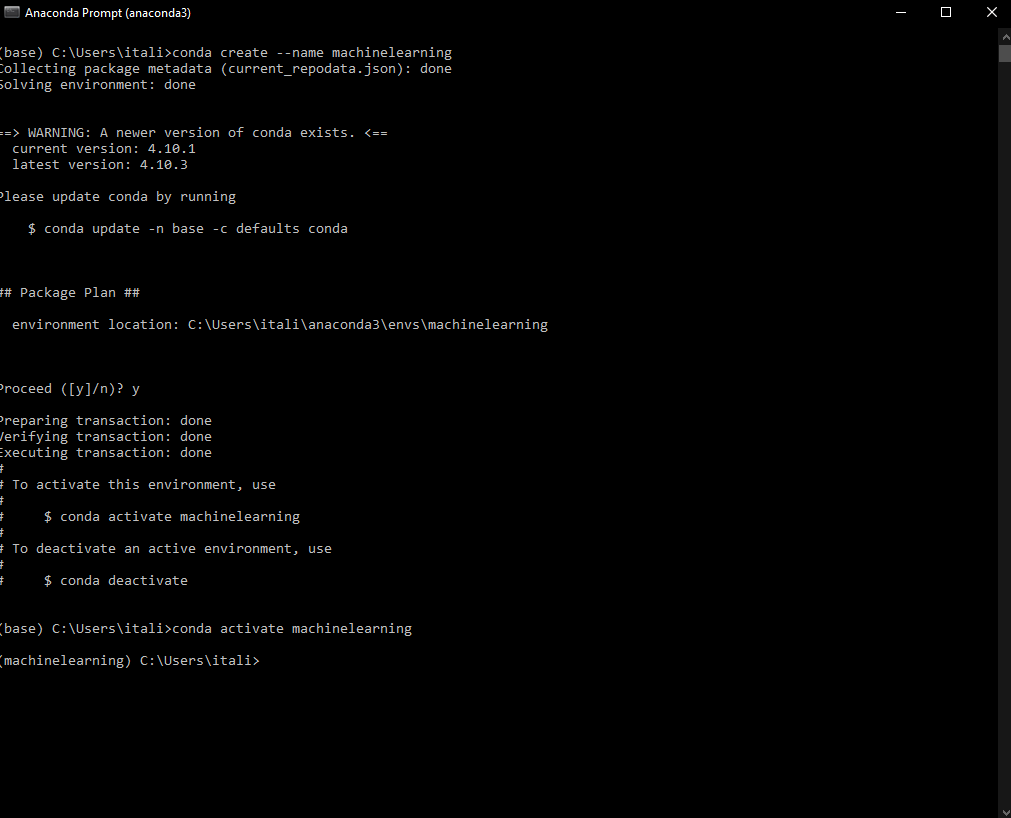
\includegraphics[width=\linewidth]{Anaconda_env.png}
  \caption{Setting up machine learning environment}
\end{figure}

These libraries are used all throughout the project as we will see later. The projects code was written within Jupyter Lab to keep all the code split into cell and have everything nice and organized.

\section{Dataset Selection}
The dataset used is the FIDS30 fruit images, I choose to select Peaches, Plums, and Mangos. These fruits have distinct physical characteristics such as color and shape that I felt would give better classification in the long run. I choose image 0 from peaches, 7 from plums, and 2 from mangos. The file directory can be seen in Figure 1.

\begin{figure}[h]
  \centering
  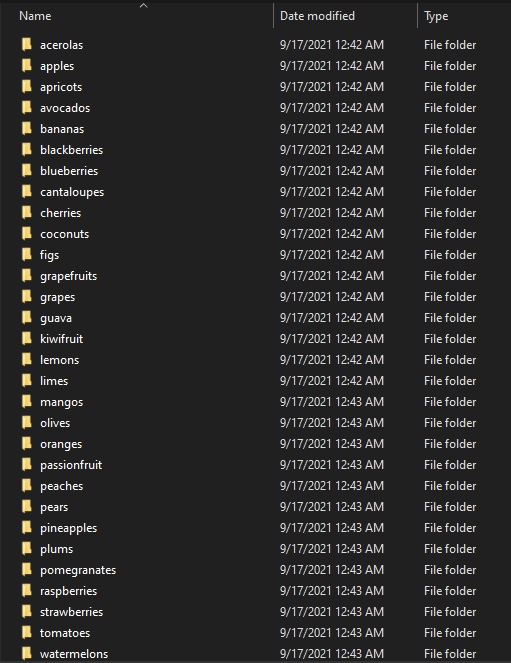
\includegraphics[width=\linewidth]{image_folder.png}
  \caption{Image of directory containing the fruit images}
\end{figure}

\section{Image Importation and Conversion}
This is where the images that are to be processes are imported using open cv along with their conversion to gray scale.

\subsection{Image Importation Code}\label{AA}
In this code (Fig.2) the images are imported in one of two ways. They are imported by a direct file path to the image or the user gives a file path with a folder of images. The images are set to a variable that is to be used later within the code.

\begin{figure}[h]
  \centering
  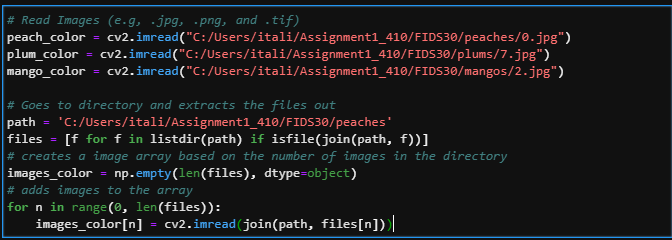
\includegraphics[width=\linewidth]{part3_code.png}
  \caption{Importation of images code}
\end{figure}

\subsection{Gray Scale Conversion}
This code takes the image that was previously obtained and converts it to gray scale using the opencv library. It then prints it shape for the user to see.

\begin{figure}[h]
  \centering
  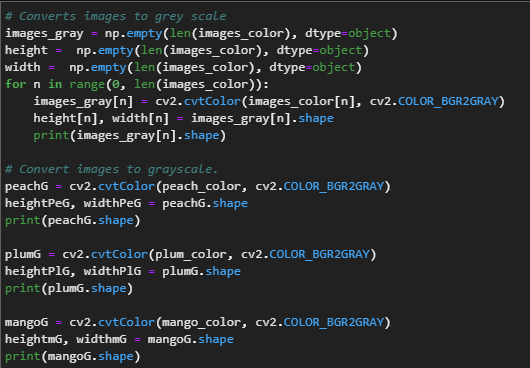
\includegraphics[width=\linewidth]{GrayScaleCode.png}
  \caption{Image Gray Scale Conversion}
\end{figure}

\section{Resizing Images}
This section takes the grayscale images and reduces their size such that they are still divisible by 8. This is so that when we extract the features later we can use our 8x8 filters.

\begin{figure}[h]
  \centering
  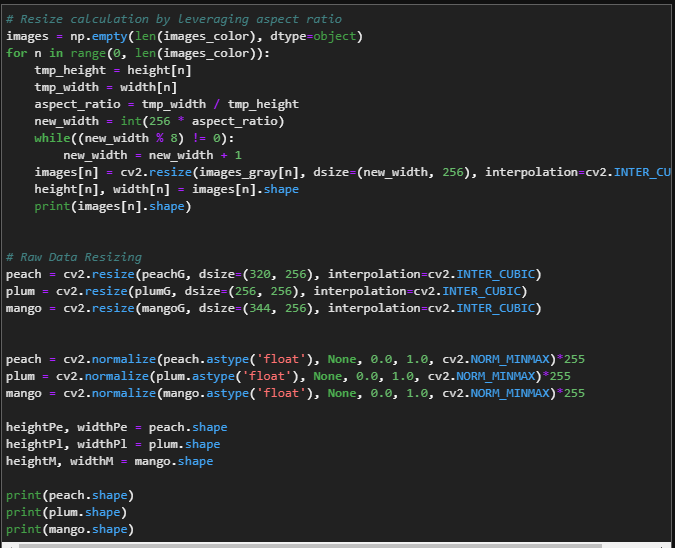
\includegraphics[width=\linewidth]{ImagesResizing.png}
  \caption{Image Resizing}
\end{figure}

The code under the comment “Resize calculation” in Fig.4 take the images from a array that were obtained from the folder given such as peaches, it then cycles through and obtains the image size. It calculates the aspect ratio, then the new width of the image based on a 256 height. Now it converts the images to their new size and saves them within a array. The bottom portion of the code is similar but only does one image at a time which is the original images selected.

\subsection{Saving the New Images}
The new images are then saved into a new folder shown in Fig.5 and Fig.6

\begin{figure}[h]
  \centering
  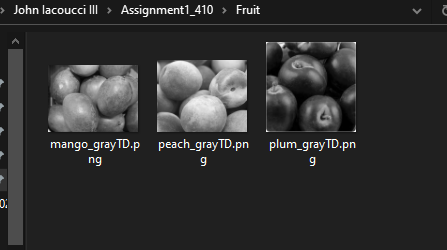
\includegraphics[width=\linewidth]{Fruit.png}
  \caption{Resized Gray Scale Images}
\end{figure}

\begin{figure}[h]
  \centering
  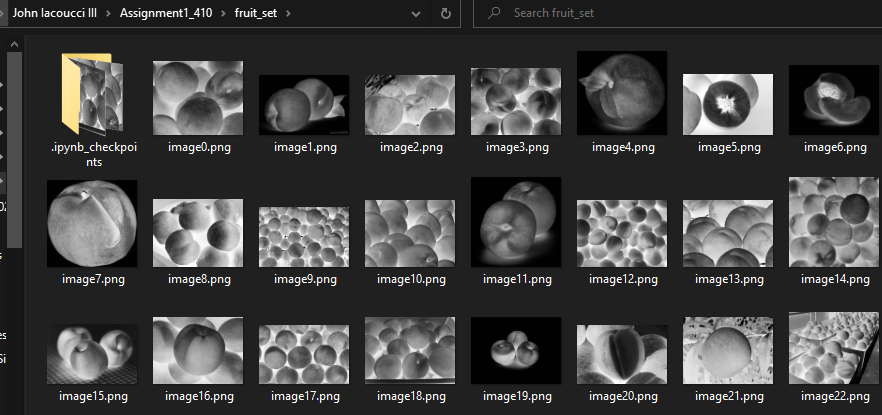
\includegraphics[width=\linewidth]{fruit_set_pic.png}
  \caption{Resized from user given a folder}
\end{figure}

\begin{figure}[h]
  \centering
  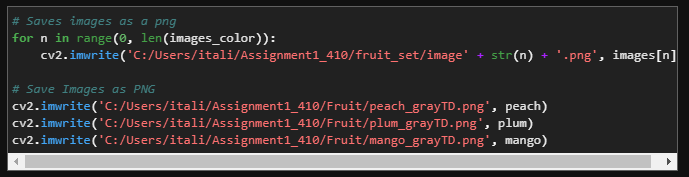
\includegraphics[width=\linewidth]{resize_save.png}
  \caption{Saving resized image}
\end{figure}

\section{Block Feature Vector}
At this point we will now take the newly created images and split them into 8x8 blocks which will extract the features from the images based on their values. They are then exported into a csv after creating a data frame using pandas.
We first binarize the images as shown in the code in Fig.8

\begin{figure}[h]
  \centering
  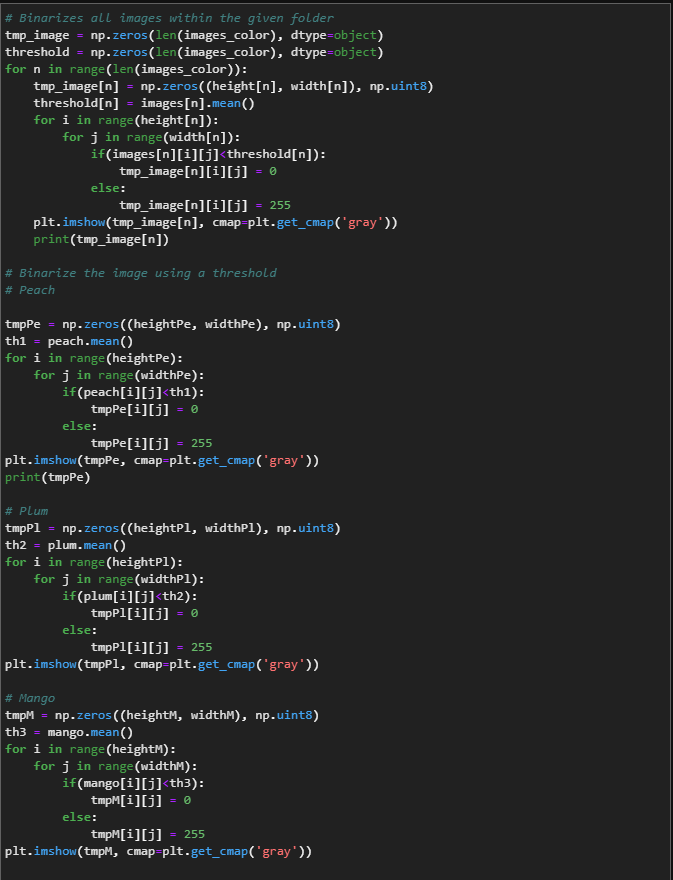
\includegraphics[width=\linewidth]{Binarize_images.png}
  \caption{Binarizing image code}
\end{figure}

This image shows both the 3 original image selections and the folder of images being binarized. We then can take our 8x8 block out of the code which is shown in Fig.9.

\begin{figure}[h]
  \centering
  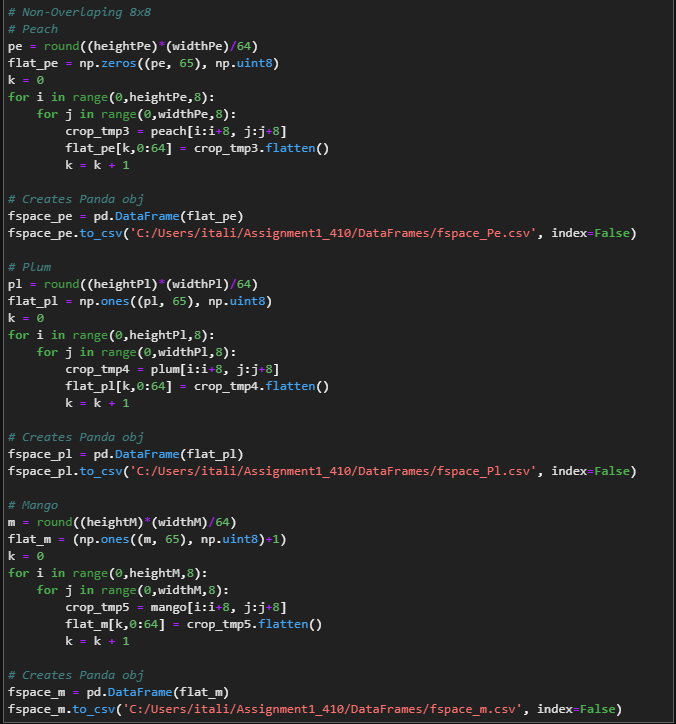
\includegraphics[width=\linewidth]{8x8NO.png}
  \caption{Non-Overlapping 8x8 Blocks}
\end{figure}

This code take the images and cycles through the values of the image to extract out the features which is then put into a data frame and exported to a csv.

\begin{figure}[h]
  \centering
  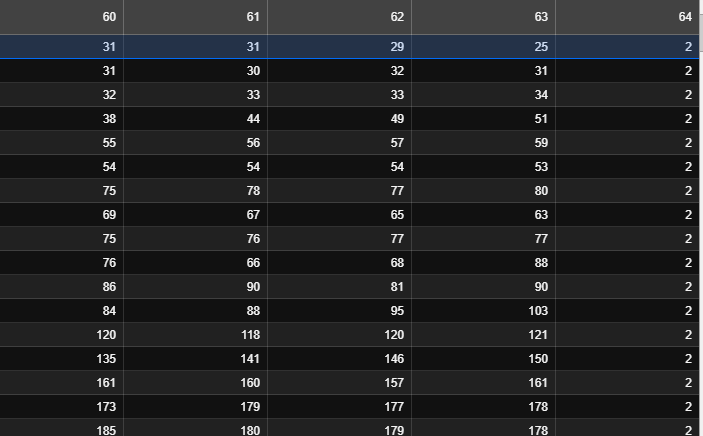
\includegraphics[width=\linewidth]{mango_dataframe.png}
  \caption{CSV of the Mango Data Frame}
\end{figure}
Fig.10 displays the mangos image data along with its classifier in column 64 which is 2.

\section{Overlapping 8X8 Block Feature Vectors}
This section is very similar to the previous section as it uses the majority of the same concept and code with a few changes.

\begin{figure}[h]
  \centering
  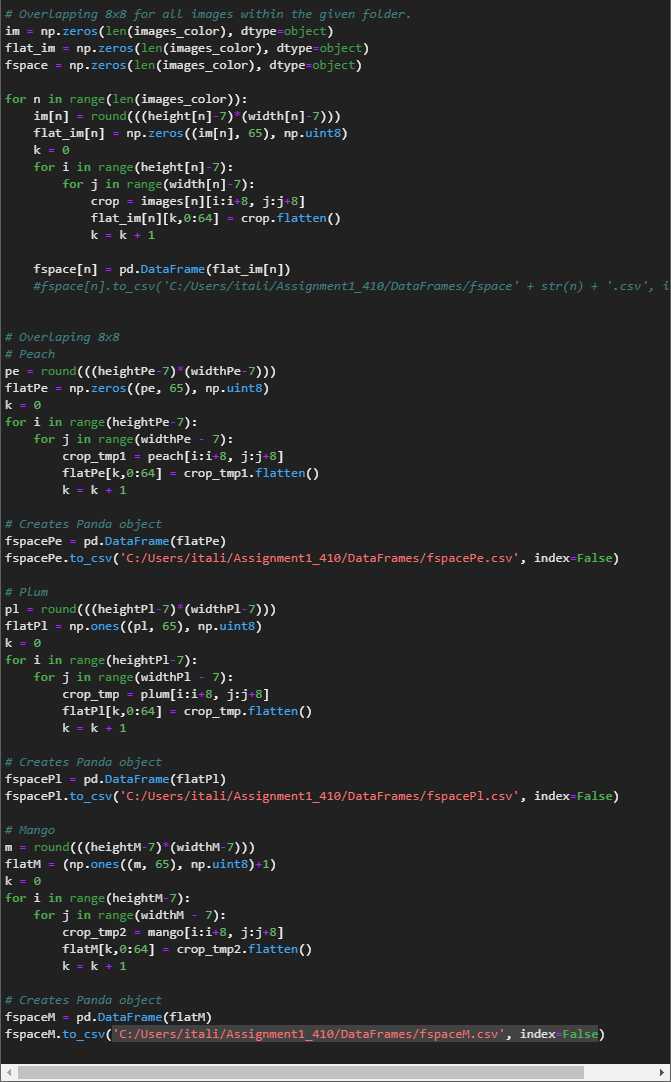
\includegraphics[width=\linewidth]{8x8ov.png}
  \caption{8x8 Overlapping Block Code}
\end{figure}
In Fig.11 the code shows that the image is being looked over by a 8x8 overlapping block so that it is only moving over one by one across the image. This allows more data to be captured that can be used in better classification later on.

\section{Statistical Data of the Images}
This data can be looked at multiple ways in which we can derive different meaning. The main things we are going to look at is if the data is balanced, accurate, and complete. The data seems to be mostly balance with the lowest observations in Fig.14 being the Plum, but it is only around 400 observations lower which should have little effect. The data is accurate since all the labels on the data is correct as we ourselves have manually assigned the labels. The data also seems complete as we can see in Fig.15. The data does not have a scalability problem as the data only has 64 features per vector which can be scaled if needed. The data is trivial as we can easily process this data with the current technology we are using now in this project. The data is also not highly dimensional since the features is not greater than the observations we have.

\begin{figure}[h]
  \centering
  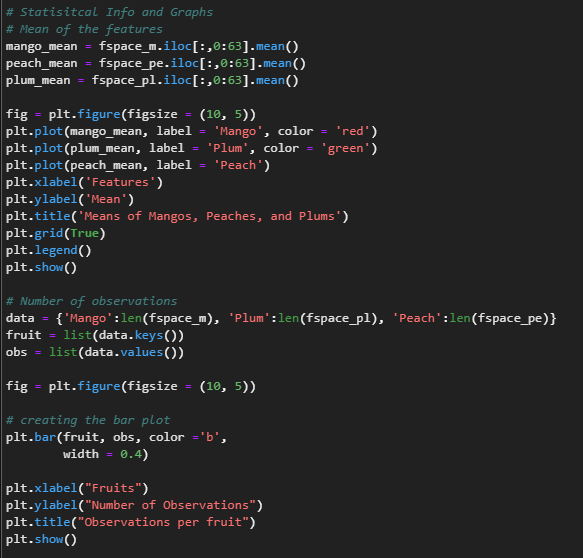
\includegraphics[width=\linewidth]{line&barplot.png}
  \caption{Statistical Graph Code}
\end{figure}

\begin{figure}[h]
  \centering
  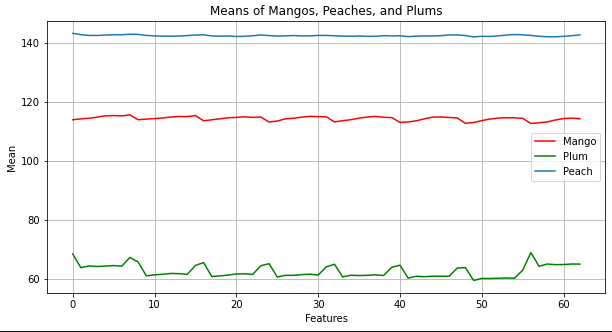
\includegraphics[width=\linewidth]{feature_means.png}
  \caption{Means of the Features per Fruit}
\end{figure}

\begin{figure}[h]
  \centering
  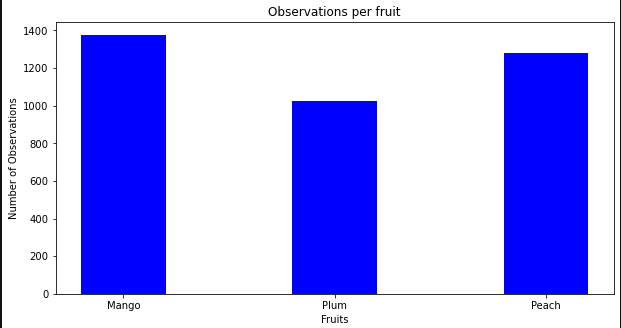
\includegraphics[width=\linewidth]{observations_fruits.png}
  \caption{Bar Graph of Observation per Fruit}
\end{figure}

\begin{figure}[h]
  \centering
  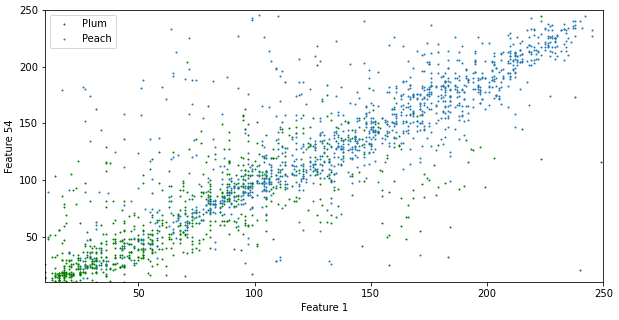
\includegraphics[width=\linewidth]{feature_peach_plum.png}
  \caption{Feature 1 and 54 from Peach and Plum Image}
\end{figure}

\section{Construct a Feature Space}
This is where everything all comes together. In the code in Fig.16 it shows the feature spaces being merged into one feature space, one is from the peaches and plums and the other is Peaches, Plums, and Mangos.

\begin{figure}[h]
  \centering
  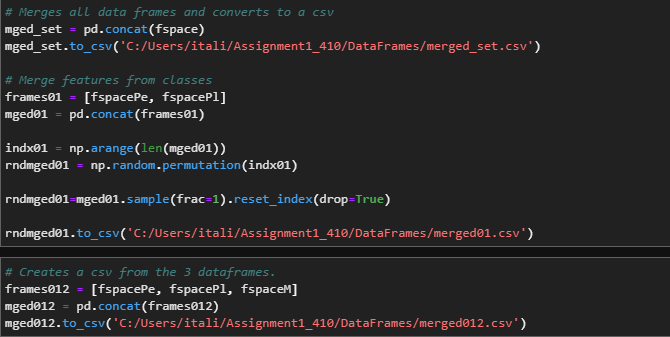
\includegraphics[width=\linewidth]{feature_space.png}
  \caption{Feature Spaces Merged}
\end{figure}

\begin{figure}[h]
  \centering
  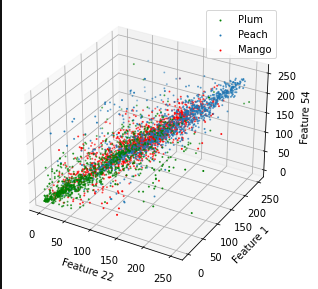
\includegraphics[width=\linewidth]{3dfeature.png}
  \caption{3d Subspace showing features 1,22,54 from the 3 fruit images}
\end{figure}

We then also randomize the feature spaces so that when we train our model is has a better learning experience.

\section{Subspace Display}
We can see the first subspace in Fig.15 which we have features 1 and 54 from the peach and plum images. The data is balanced and accurate as the data is spread out. This is taken from the data frame of the non overlapping 8x8 blocks.


This is the 3d subspace where we get a better idea of the positioning of the data and how it orients itself. We can change the features around such that we could get different angles to view the data to see how the data could be classified. Compared to Fig.15 we get a slightly better idea of how to classify the data but the data is still very much intertwined which could make it hard to classify for a model. We would need to apply some changes to the data sets to get better result before being able to give this to a model. This is the code used to create said graph.

\begin{figure}[h]
  \centering
  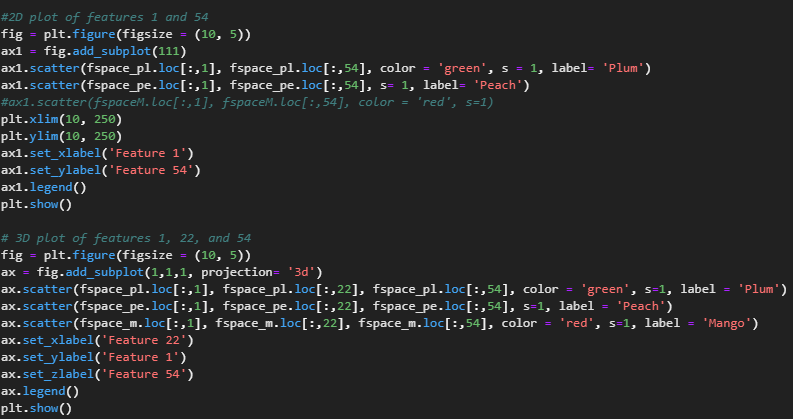
\includegraphics[width=\linewidth]{2d_3d_code.png}
  \caption{2D, 3D Graph Code}
\end{figure}

\section{Additional Code}
The additional code which makes the program more modular is given throughout the figures previously discussed. This code allows a folder to be given and turned into a feature space within a csv file. This code is using the peaches folder so all images are similar and the classifier will be the same this can be helpful when large amounts of similar data needs to be obtained.

\section{Effects of Block Size}
The block size chosen is 8x8 which would give is a dimensionality of 64 and or 64 features. This is a relatively low number of features for data that is going to be used to train models. Also depending on if the data is overlapping or not the blocks limit us to a certain number of vectors. If we were to reduce the filter size it would allow us to capture more local information that would allow us to better classify the images. With the current data from the images using this 8x8 block it is going to be difficult to classify the images based on the domain of data.

\section{Dividing the Domain}
To start the data collected from the previous assignment was used to train the models that will be discussed later-on. In order to get the data sets to train and test these models I wrote a function that takes a file name specifically a csv and splits the data into a 80:20 split 80 percent will go to training and the other 20 percent will go to testing. Furthermore, I separated the training and testing into the x and y portions of each data set. Then taking each x and y for testing and training and exporting them as their own csv files to be used for training and testing later.

The splitting was done using the sklearn library using the split function which takes the output variables as arguments along with the data set to be split, the function also can be customized and be told what percent of data you want to use for testing. In this case the parameter was set to 0.2 for 20 percent testing data.

\section{Relation between Training and Testing Data Sets}
\begin{figure}[h]
  \centering
  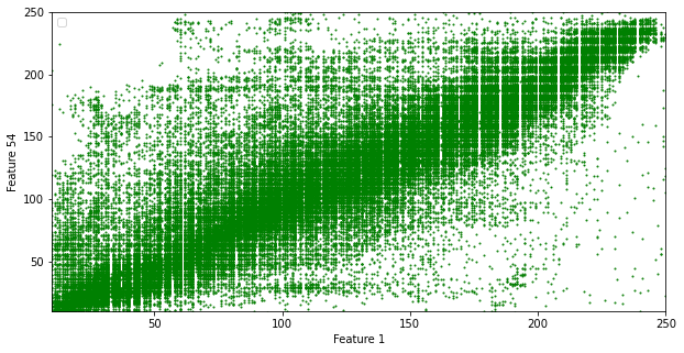
\includegraphics[width=\linewidth]{trainingSp.png}
  \caption{Scatter Plot of Training Data}
\end{figure}

\begin{figure}[h]
  \centering
  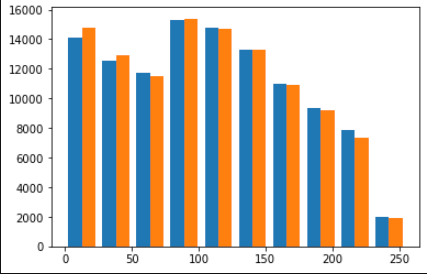
\includegraphics[width=\linewidth]{trainingHis.png}
  \caption{Histogram of Training Data}
\end{figure}

\begin{figure}[h]
  \centering
  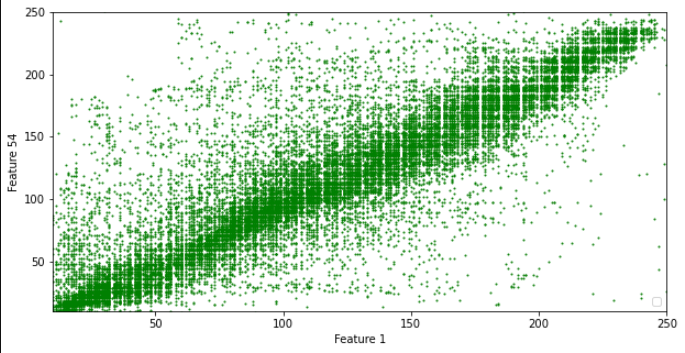
\includegraphics[width=\linewidth]{testsp.png}
  \caption{Scatter Plot of Testing Data}
\end{figure}

\begin{figure}[h]
  \centering
  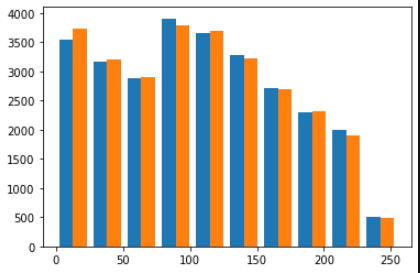
\includegraphics[width=\linewidth]{testingHis.png}
  \caption{Histogram of Testing Data}
\end{figure}

We can look at Fig.20 and 22 to see that both follow the same distribution but with the training data being much more dense. In Fig.21 and 23 we can also see that they follow the same distributions as they are both skewed to the right.

\section{Elastic-Net Regression Model}
Now we move onto developing the model, in this case we are using a regression model which is the elastic-net model. In this model we are taking the training and testing data sets we created earlier and importing them in. We assign the training values x and y to their respective variables and the testing x and y as well. The regression model is done using the sklearn library and takes the training values as parameters. We then create a new variable to hold the predictions and assign the x testing values to to make the predictions. This is then entered into a confusion matrix which takes the y testing values and the predicted values to determine which data points were classified correctly. In the confusion matrix found below you can see that we had 12651 classified as label 0 correctly and 9457 classified as label 1 correctly. This gave and accuracy of 0.7899 and a precision of 0.7643. These numbers are ok for a regression model and could be possibly improved with optimizing our parameters.

\begin{figure}[h]
  \centering
  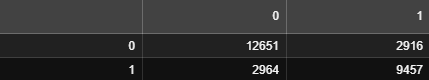
\includegraphics[width=\linewidth]{confusionElastic.png}
  \caption{Confusion Matrix for Elastic-Net Regression Model}
\end{figure}

\begin{figure}[h]
  \centering
  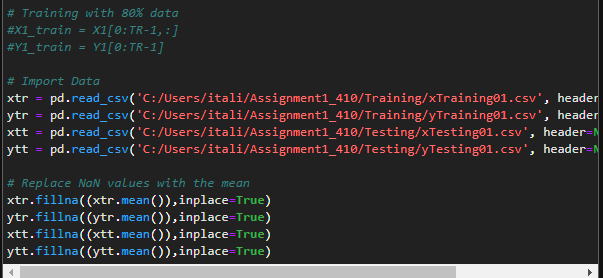
\includegraphics[width=\linewidth]{elasticNetImport.png}
  \caption{Imports for Elastic-Net Model}
\end{figure}

\begin{figure}[h]
  \centering
  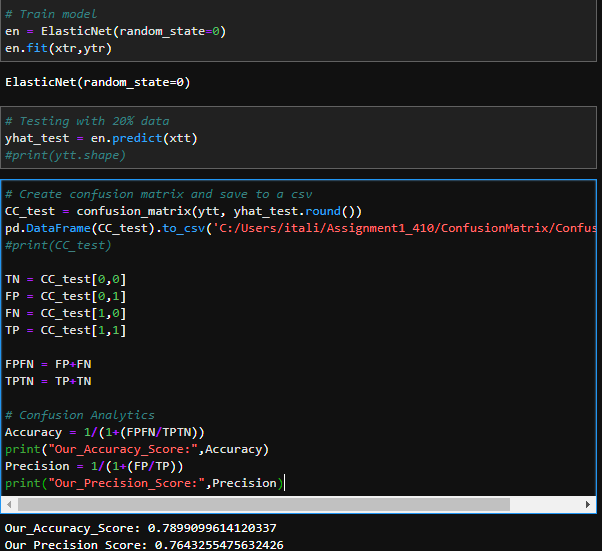
\includegraphics[width=\linewidth]{elasticNetTraining.png}
  \caption{Elastic Net Training}
\end{figure}

\section{Random Forest}
The random forest model is a bit more complex by using multiple decision trees to reach a decision or result. It is more accurate as we will see from the results obtained. The data is once again imported in using the pandas library into a data frame and split between the x and y training and testing variables. The training variables are then put into the model to be trained. This training is slightly different because it uses ensembles as shown in the figures below to take the most popular result which uses bootstrap aggregation. It then takes the x testing values and tests the model. Again using a confusion matrix it gives 15236 points classified as label 0 correctly and 11761 points classified as label 1 correctly as seen in the figure below. This gives a accuracy of 0.9646 and a precision of 0.9726 both are much higher than the previous model.

\begin{figure}[h]
  \centering
  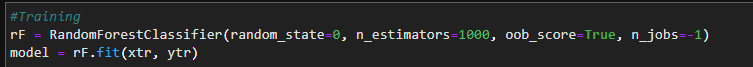
\includegraphics[width=\linewidth]{RFT.png}
  \caption{Random Forest Training}
\end{figure}

\begin{figure}[h]
  \centering
  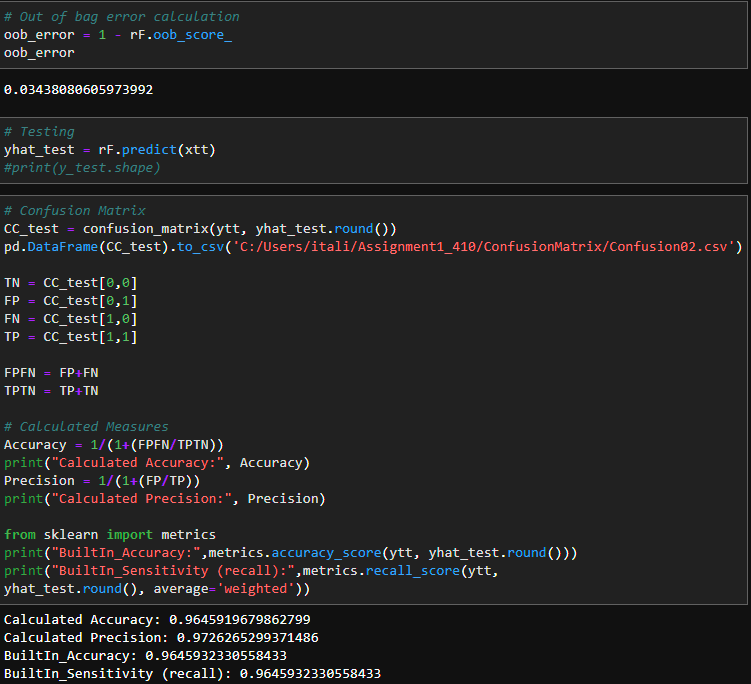
\includegraphics[width=\linewidth]{RFCode.png}
  \caption{Random Forest Code}
\end{figure}

\section{Comparing the Models}
The models can be compared using a function of the sklearn library which is the metrics accuracy and sensitivity functions. The builtin function measured the elastic-nets accuracy and sensitivity at 0.7898 and 0.7898. The random forest builtin accuracy and sensitivity measured at 0.9646 and 0.9646. This shows that the random forest model is much more accurate at predicting the class and with a higher sensitivity it also has a greater chance of identifying the correct labels.

The differences with the confusion matrix compared to the regular quantitative measure is largely in part from its ability to understand the data better while giving feed back to the engineer. The confusion matrix has the ability to determine the positives and false positives of the models predictions. This will allow the engineer to have insight to what the model is predicting and be able to better fix the issues with the model. Compared to the regular measures that will only provide feedback on as specific thing like accuracy. Knowing whether the accuracy is high or low is useful but being able to tell that label 1 has much higher false positives will give the extra advantage in fixing or optimizing the model.

The random forest model is by far the better model than the elastic-net. The model not only had higher accuracy in both the builtin and confusion matrix but also with the precision of the model compared 0.97 to 0.76. This model also has less false positives compared to the elastic-net with a total of 991 to 5880, this model can also be used for multiple classification situations compared to the regression only being optimal for two class scenarios.

\section{Big Data System}
The big data system is used to process the large amounts of data from the fruit images and more efficiently train machine learning models like we will see later on.

\subsection{Getting Familiar with Databricks}
The big data system I used was Databricks, to start I signed up for a community edition account and started the quick-start tutorial along with watching Dr.Suthaharan video. The quick start tutorial showed how to create a new cluster which was done by going to the compute tab and clicking the create a cluster button. I then selected the type of environment to run the notebook in and created the cluster which took roughly 10 minutes to create. The tutorial then showed me how to detach and attach the notebook to the newly created cluster and run everything. A important part of the tutorial is in the code provided within the notebook, the query to the data table in order to convert the table into a data frame using spark is a important step as we will see later on. The query is identical to a SQL query so even though I just queried the entire table I can see how being able to query the data in anyway can be extremely useful.

\subsection{Setting up the Environment}
The environment setup was exactly the same as in the tutorial, I created a new cluster called FruitCluster with the 7.3 LTS ML version that runs Spark 3.0.1 and Scala 2.12. Then I began to import the data sets into databricks, to do so I went to the data tab on the left side and clicked create table. From there I loaded the csv file from the data frame into databricks and clicked create table with UI with the cluster I created before. Then after changing the settings to first row is header, infer schema to on I created the table. This turned the data into a database table which can now be used to query.

\begin{figure}[h]
  \centering
  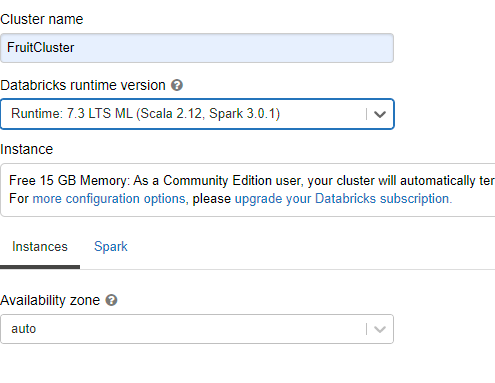
\includegraphics[width=\linewidth]{cluster_creation.png}
  \caption{Cluster Creation}
\end{figure}

\begin{figure}[h]
  \centering
  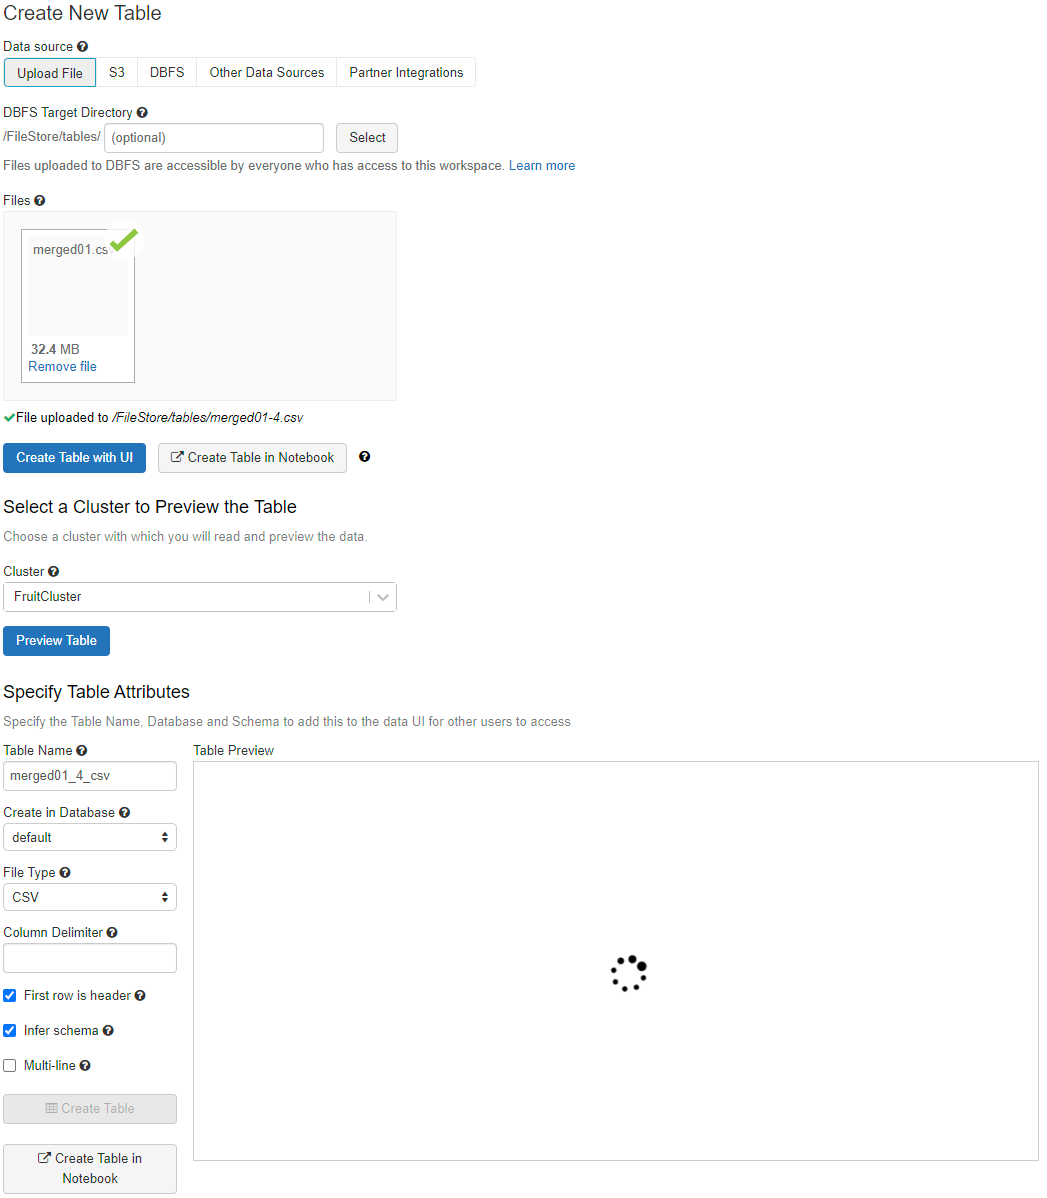
\includegraphics[width=\linewidth]{datatable_creation.png}
  \caption{Database Creation}
\end{figure}

\section{Training Random Forest with Databricks}
The training of the random forest model was fairly straight forward as I followed the tutorial given within the assignment. I started with importing the previously created database and converted it to a dataframe using pandas. Next I checked for any NaN values and split the dataframe 80:20 for the training and testing using the sklearn train test split function. Then I created the random forest model by using mlflow which will allow for each iteration of the model to become an experiment that can be analyzed and used to save the model for later use. This is also where the auc score is calculated which is also logged by mlflow. After the model was trained and tested within the last function I calculated displayed the important features then displayed the auc score for that experiment.

\begin{figure}[h]
  \centering
  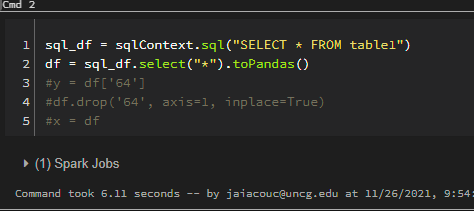
\includegraphics[width=\linewidth]{sql_import.png}
  \caption{Sql Import}
\end{figure}

\section{Results}
In this section I will talk about the results obtained from the new databricks model. Also I will compare the databricks model to the previous model computed on the local machine.

\subsection{Results from Databricks}
The Databricks experiment showed the following, the auc was 0.987 which means that the model predicted the data accurately and with a time of only 9 seconds. This is lighting fast for a random forest algorithm as we will see later. I also saw from computing the important features that feature 49 had the most impact among the other features.

\subsection{Comparing Databricks to Local Machine}
The accuracy of the models were fairly close with the databricks model being slightly more accurate with .98 compared to the local machines .96. The thing that shows how effective the big data system was though was in the computational time the local machine took 2 minutes to complete the training of the random forest model compared to the big data systems 9 seconds. This difference is huge although 2 minutes isn't a lot of time, if the data set was even larger than this one then the local machine would not even be able to process it while the big data system could still process and train the model within a reasonable time frame.

\begin{figure}[h]
  \centering
  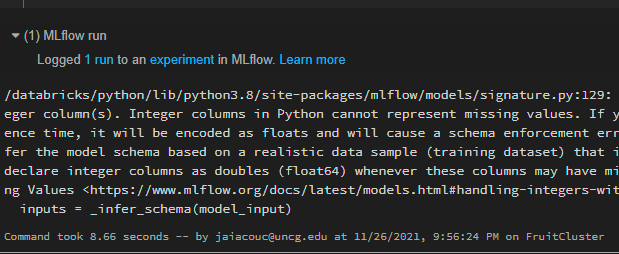
\includegraphics[width=\linewidth]{DB_RF_time.png}
  \caption{Databricks Computation Time}
\end{figure}

\begin{figure}[h]
  \centering
  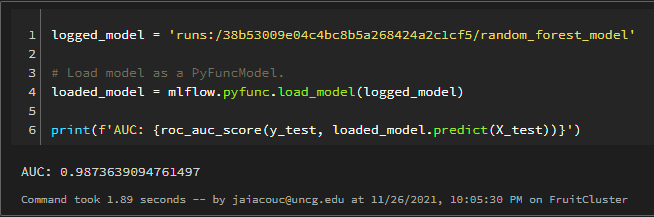
\includegraphics[width=\linewidth]{auc_score.png}
  \caption{Auc Score}
\end{figure}

\begin{thebibliography}{00}
\bibitem{b1} Automatic fruit recognition using computer vision, Škrjanec Marko, Bsc Thesis, (Mentor: Matej Kristan), Fakulteta za računalništvo in informatiko,Univerza v Ljubljani, 2013

\end{thebibliography}
\end{document}
